\section{Sequências}
   \subsection{A reta real estendida}
      Existem algumas sequências que não convergem para um número 
      real e dependendo de como é a sua lei de formação podemos 
      enxergar isso. Essas sequências convergem para $+\infty$ ou 
      $-\infty$. Talvez seja adequado dizer que a sequência 
      $$1,2,3,4,5,...$$ esteja convergindo para $+\infty$, 
      enquanto $$-1,-2,-3,-4,-5,...$$ esteja convergindo 
      para $-\infty$.
      \begin{definition}[Reta real estendida]
         A reta real estendida $\mathbf{R*}$ é a reta real $\R$ com dois elementos 
         distintos de qualquer outro elemento de $\R$.
         $$\mathbf{R*} := \R \cup \{-\infty,+\infty\}$$
      \end{definition}
      \begin{definition}[Supremo]
         Seja $E$ um subconjunto dos números reais. Se $E$ é não vazio 
         e tem algum limite superior, definimos $sup(E)$ como o 
         limite superior mínimo de $E$ (o menor dos limites superiores de $E$, e, 
         também, ele é único).\\
         Se $E$ é um conjunto não vazio e não tem um limite superior, o 
         $sup(E) := +\infty$. Se $E$ for vazio temos $sup(E) := -\infty$.
      \end{definition}

      \tikzset{every picture/.style={line width=0.75pt}}
      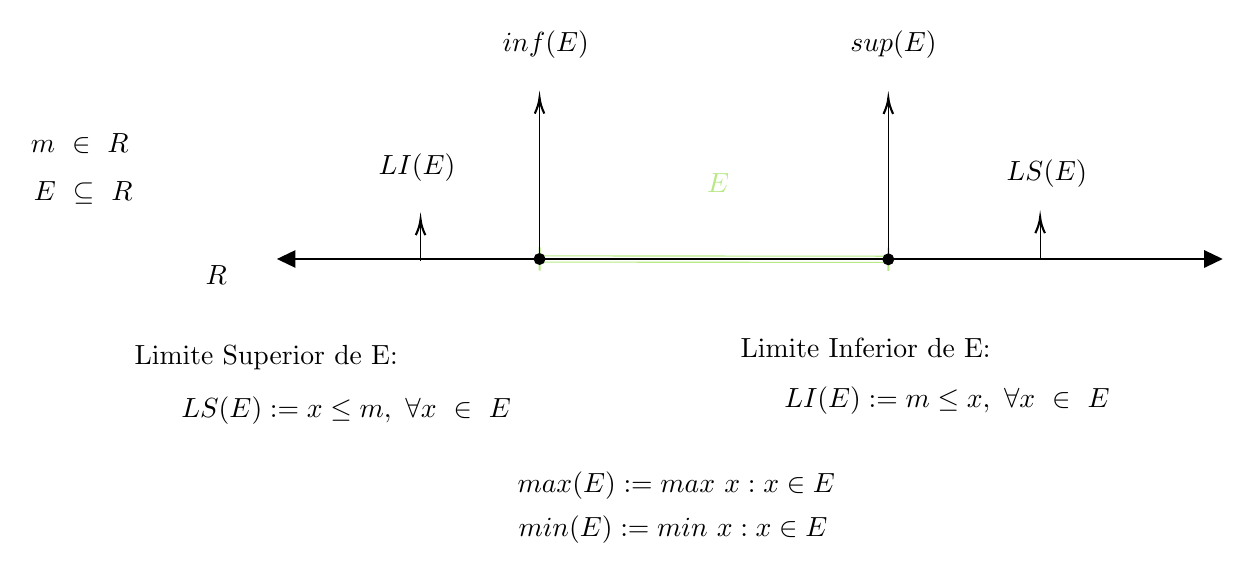
\begin{tikzpicture}[x=0.75pt,y=0.75pt,yscale=-1,xscale=1]
         \draw    (524.53,130.92) -- (524.53,112.81) ;
         \draw [shift={(524.53,110.81)}, rotate = 90] [color={rgb, 255:red, 0; green, 0; blue, 0 }  ][line width=0.75]    (7.65,-2.3) .. controls (4.86,-0.97) and (2.31,-0.21) .. (0,0) .. controls (2.31,0.21) and (4.86,0.98) .. (7.65,2.3)   ;
         %Straight Lines [id:da22070511664638137] 
         \draw [color={rgb, 255:red, 184; green, 233; blue, 134 }  ,draw opacity=1 ]   (451.38,132.58) -- (283.35,132.42)(451.39,129.58) -- (283.35,129.42) ;
         \draw [shift={(283.35,130.92)}, rotate = 0.05] [color={rgb, 255:red, 184; green, 233; blue, 134 }  ,draw opacity=1 ][line width=0.75]    (0,5.59) -- (0,-5.59)   ;
         \draw [shift={(451.39,131.08)}, rotate = 0.05] [color={rgb, 255:red, 184; green, 233; blue, 134 }  ,draw opacity=1 ][line width=0.75]    (0,5.59) -- (0,-5.59)   ;
         %Straight Lines [id:da22510211195741192] 
         \draw [fill={rgb, 255:red, 208; green, 2; blue, 27 }  ,fill opacity=1 ]   (159.83,130.92) -- (476.1,130.92) -- (600.64,130.92) -- (609.5,130.92) ;
         \draw [shift={(612.5,130.92)}, rotate = 180] [fill={rgb, 255:red, 0; green, 0; blue, 0 }  ][line width=0.08]  [draw opacity=0] (8.93,-4.29) -- (0,0) -- (8.93,4.29) -- cycle    ;
         \draw [shift={(156.83,130.92)}, rotate = 0] [fill={rgb, 255:red, 0; green, 0; blue, 0 }  ][line width=0.08]  [draw opacity=0] (8.93,-4.29) -- (0,0) -- (8.93,4.29) -- cycle    ;
         %Straight Lines [id:da8812203543817227] 
         \draw    (451.39,131.08) -- (451.39,55.37) ;
         \draw [shift={(451.39,53.37)}, rotate = 90] [color={rgb, 255:red, 0; green, 0; blue, 0 }  ][line width=0.75]    (7.65,-2.3) .. controls (4.86,-0.97) and (2.31,-0.21) .. (0,0) .. controls (2.31,0.21) and (4.86,0.98) .. (7.65,2.3)   ;
         \draw [shift={(451.39,131.08)}, rotate = 270] [color={rgb, 255:red, 0; green, 0; blue, 0 }  ][fill={rgb, 255:red, 0; green, 0; blue, 0 }  ][line width=0.75]      (0, 0) circle [x radius= 2.34, y radius= 2.34]   ;
         %Straight Lines [id:da00885463066681158] 
         \draw    (226.02,131.88) -- (226.02,113.77) ;
         \draw [shift={(226.02,111.77)}, rotate = 90] [color={rgb, 255:red, 0; green, 0; blue, 0 }  ][line width=0.75]    (7.65,-2.3) .. controls (4.86,-0.97) and (2.31,-0.21) .. (0,0) .. controls (2.31,0.21) and (4.86,0.98) .. (7.65,2.3)   ;
         %Straight Lines [id:da503391711573659] 
         \draw    (283.35,130.92) -- (283.35,55.21) ;
         \draw [shift={(283.35,53.21)}, rotate = 90] [color={rgb, 255:red, 0; green, 0; blue, 0 }  ][line width=0.75]    (7.65,-2.3) .. controls (4.86,-0.97) and (2.31,-0.21) .. (0,0) .. controls (2.31,0.21) and (4.86,0.98) .. (7.65,2.3)   ;
         \draw [shift={(283.35,130.92)}, rotate = 270] [color={rgb, 255:red, 0; green, 0; blue, 0 }  ][fill={rgb, 255:red, 0; green, 0; blue, 0 }  ][line width=0.75]      (0, 0) circle [x radius= 2.34, y radius= 2.34]   ;

         % Text Node
         \draw (121.16,132.71) node [anchor=north west][inner sep=0.75pt]    {$\mathbb{R}$};
         % Text Node
         \draw (37,69.4) node [anchor=north west][inner sep=0.75pt]    {$m\ \in \ \mathbb{R}$};
         % Text Node
         \draw (38.5,92.4) node [anchor=north west][inner sep=0.75pt]    {$E\ \subseteq \ \mathbb{R}$};
         % Text Node
         \draw (362.85,88.67) node [anchor=north west][inner sep=0.75pt]  [color={rgb, 255:red, 184; green, 233; blue, 134 }  ,opacity=1 ]  {$E$};
         % Text Node
         \draw (109.5,195.9) node [anchor=north west][inner sep=0.75pt]    {$LS( E) :=x\leq m,\ \forall x\ \in \ E$};
         % Text Node
         \draw (87,171) node [anchor=north west][inner sep=0.75pt]   [align=left] {Limite Superior de E:};
         % Text Node
         \draw (506.63,81.97) node [anchor=north west][inner sep=0.75pt]  [xslant=-0.04]  {$LS( E)$};
         % Text Node
         \draw (379,168) node [anchor=north west][inner sep=0.75pt]   [align=left] {Limite Inferior de E:};
         % Text Node
         \draw (400,191.4) node [anchor=north west][inner sep=0.75pt]    {$LI( E) :=m\leq x,\ \forall x\ \in \ E$};
         % Text Node
         \draw (204.55,79.1) node [anchor=north west][inner sep=0.75pt]    {$LI( E)$};
         % Text Node
         \draw (431.83,19.74) node [anchor=north west][inner sep=0.75pt]    {$sup( E)$};
         % Text Node
         \draw (264.29,19.74) node [anchor=north west][inner sep=0.75pt]    {$inf( E)$};
         % Text Node
         \draw (271.5,232.4) node [anchor=north west][inner sep=0.75pt]    {$max( E) :=max\ x:x\in E$};
         % Text Node
         \draw (272,253.4) node [anchor=north west][inner sep=0.75pt]    {$min( E) :=min\ x:x\in E$};
      \end{tikzpicture}

      \begin{definition}[Supremo do conjunto de reais estendidos]
         Seja $E$ um subconjunto de $\mathbf{R*}$. Então definimos o 
         \emph{supremo} $sup(E)$ como 
         \begin{enumerate}[(a)]
            \item 
               Se $E$ esta contido em $\R$ ($\{-\infty,+\infty\}) \notin E$) 
               então $sup(E)$ é definido da forma usual (definição 
               de supremo acima).
            \item
               Se $E$ contem $+\infty$, então $sup(E) := +\infty$.
            \item
               Se $E$ não contem $+\infty$ mas contem $-\infty$, então 
               $$sup(E):= sup(E\setminus \{-\infty\}).$$ Mas isso 
               é um subconjunto de $\R$ e, então, cai no item (a).
         \end{enumerate}
         Como visto na figura acima também temos o \emph{ínfimo} $inf(E)$. 
         O ínfimo de $E$ é o maior numero do limite inferior.
         $$inf(E):=-sup(-E).$$
      \end{definition}
      \begin{exmp}
         Seja $E$ os inteiros negativos, juntos com $-\infty$:
         $$E = \{-1,-2,-3,-4,...\}\cup \{-\infty\}.$$
         Assim $$sup(E) = sup(E\setminus \{-\infty\}) = -1,$$
         enquanto $inf(E) = -sup(-E)=-(+\infty)=-\infty$.
      \end{exmp}
      \begin{stat}
         Seja $E$ um conjunto vazio. Então $sup(E) = -\infty$ e 
         $inf(E) = +\infty$.
      \end{stat}
      Este é o único caso onde o supremo é menor que o ínfimo.\\
      Imaginando uma reta real com $+\infty$ para a direita e $-\infty$ 
      para a esquerda. Movendo-se de $+\infty$ para a esquerda 
      ate parar quando encontrar o conjunto $E$. Esse local de parada 
      é o supremo de $E$. Analogamente movendo-se de $-\infty$ para 
      a direita ate encontrar o conjunto $E$; o local de parada será 
      o ínfimo de $E$. No caso de $E$ ser um conjunto vazio não 
      haverá local de parada e os "pontos" se movendo na reta 
      irão para direções opostas. Portanto, o supremo se torna 
      $-\infty$ e o ínfimo $+\infty$.
   \subsection{Sequências infinitas}
      Sequências são um tipo de especial de função. 
      Considere uma função de variável inteira, ou seja, 
      $$a_{n} := a(n): \Z \to A; n\ \mapsto\ a_{n}.$$
      O domínio de uma sequência é sempre o conjunto dos inteiros. 
      A imagem da sequência depende do contexto, pois o 
      contradomínio pode ser um subconjunto do conjunto 
      $\R$, $\C$ ou um espaço topológico. 
      De qualquer forma, a imagem é geralmente denotada por $a_{n}$.
      \subsubsection{Sequências infinitas unilaterais}
          São sequências onde o domínio pode ser sempre o conjunto $\N$. 
          Considere a aplicação $f: N \to A; n \mapsto f(n).$ 
          Uma sequência infinita unilateral seria algo do tipo 
          $$\left\{a_{n}\right\}^{\infty}_{n \in \N}.$$
         \begin{exmp}
            Considere a sequência $\left\{\cos{\dfrac{n\pi}{6}}\right\}
            ^{\infty}_{n=0}$. Então, a imagem é $\left\{1,
            \dfrac{\sqrt[]{3}}{2}, \dfrac{1}{2}, ...\right\}.$
         \end{exmp}
      
      \subsubsection{Sequências bi-infinitas}
         Sequências bi-infinitas são sequências do tipo 
         $$\left\{a_{n}\right\}^{\infty}_{n=-\infty}.$$
         \begin{exmp}
            Considere $\left\{4n\right\}^{\infty}_{n=-\infty}$. 
            Então, temos $$(..., -16,-12,-8,-4,0,4,8,12,16,...).$$
         \end{exmp}
   \subsection{Sequências monótonas}
      Sequências monótonas são sempre crescentes ou decrescentes. 
         \subsubsection{Sequências monotonicamente crescentes}
               A sequência $\left\{a_{n}\right\}^{\infty}_{n=1}$ 
               é monotonicamente crescente se e somente se 
               $a_{n+1} \geq a_{n}$, para todo $n \in \N$. 
               Se cada termo consecutivo é estritamente maior que o 
               anterior, então a sequência é \emph{estritamente 
               monotonicamente crescente}.
            \subsubsection{Sequências monotonicamente decrescentes}
               Analogamente, uma sequência é monotonicamente decrescente 
               se a cada termo consecutivo for menor que o anterior. 
               A sequência será \emph{estritamente monotonicamente 
               decrescente} se cada termo for estritamente menor que o anterior.
      
   \subsection{Sequências limitadas}
      \begin{definition}
         Uma sequência $\left\{a_{n}\right\}^{\infty}_{n \in A}$
         é limitada quando o conjunto de seus termos é limitado, 
         ou seja, existem $K$ e $M$ contidos em $A$ tais que 
         $K \leq a_{n} \leq M, \forall n \in A$.
         \begin{enumerate}[i.]
            \item Se $\left\{a_{n}\right\}$ é limitada superiormente 
               temos $$a_{n} \leq M,\forall n \in A.$$
            \item Se $\left\{a_{n}\right\}$ é limitada inferiormente 
               temos $$K \leq a_{n}, \forall n \in A.$$
            \item Se $\left\{a_{n}\right\}$ é inferiormente e superiormente
               limitada então $\left\{a_{n}\right\}$ é uma sequência limitada.
               Isto é, ${a_{n}}$ é limitada se existir um 
               $L > 0$, $L \subseteq A$, tal que 
               $|a_{n}| \leq L, \forall n \in A$.
         \end{enumerate}
      \end{definition}
      \begin{lemma}[Sequências finitas são limitadas]
         Toda sequência finita $a_{1},a_{2},...,a_{n}$ é limitada.
         \begin{proof}
            Por indução, primeiramente, temos que quando $n=1$ a 
            sequência $\{a_{1}\}$ é claramente limitada, pois se 
            escolhermos $M := |a_{1}|$ então temos 
            $|a_{i}| \leq M$ para todo $1 \leq i \leq n$. Agora 
            suponha que ja provamos o lema para algum $n \geq 1$; 
            agora temos que provar isso para $n++$, i.e, nos temos 
            que provar que toda sequência $\{a_{i}\}^{n++}_{i=1}$ 
            é limitada. Pela hipótese da indução temos que 
            $a_{1},a_{2}, ...,a_{n}$ é limitada por algum $M \geq 0$.
            Em particular, queremos a limitação por 
            $M + |a_{n++}|$. Por outro lado, $\{a_{n++}\}$ 
            também é limitada por $M + |a_{n++}|$.
            Assim $a_{1},a_{2},...,a_{n},a_{n++}$ é limitada 
            por $M + |a_{n++}|$. Isso termina a indução em $n$.
         \end{proof}
      \end{lemma}
   \subsection{Limite de uma sequência}
      Sequências são tipos especiais de funções e com isso podemos 
      investigar seus limites. No entanto, temos uma restrição: 
      ${a_{n}}$ está definida para valores inteiros de $n$. 
      O único limite que usado será de $a_{n} \to +\infty.$
      \begin{definition}[Intuitiva]
         Dada uma sequência ${a_{n}}$ dizemos que o limite de uma sequência é
         $L$ se, enquanto $n$ se torna grande, $a_{n}$ começa a estar
         arbitrariamente perto de $L$. Se enquanto 
         $n \to +\infty$ $a_{n}$ não
         se aproxima de $L$, então dizemos que o limite não existe.
      \end{definition}
      \begin{definition}
         Dada uma sequência ${a_{n}}$ dizemos que 
         $\lim_{n\to\infty} a_{n} = L$ se para todo 
         $\epsilon > 0$ existir um inteiro $k$, tal que $| a_{n} -
         L | < \epsilon$ para todo $n \geq k$.
      \end{definition}
      \begin{theorem}
         Seja ${a_{n}}_{n=n_{0}}$ uma sequência e suponha que $f(x)$ é uma
         função real para a qual $f(n) = a_{n}$ para todos os inteiros $n \geq k$,
         onde $k \geq n_{0}$. Se $$\lim_{x\to\infty} f(x) = L,\quad
         \lim_{n\to\infty} a_{n} = L.$$
      \end{theorem}
      \begin{exmp}
         Seja $a_{n} = \dfrac{5n+1}{6n+7}$. Determine se a sequência
         ${a_{n}}_{n=1}$ tem um limite.
         \begin{proof}
            Como $$\lim_{x\to\infty} \dfrac{5x+1}{6x+7} = 
            \dfrac{5}{6},\quad \textrm{então}\ \lim_{x\to\infty} 
            \dfrac{5n+1}{6n+7} = \dfrac{5}{6}.$$
         \end{proof}
      \end{exmp}
      \begin{mymdframed}{Observação}
         Se $\lim_{x\to\infty} f(x)$ não existe, 
         $\lim_{n\to\infty} a_{n}$ pode não existir.
      \end{mymdframed}
      \begin{exmp}
         Considere $a_{n} = \sin(n\pi)$ e $f(x) = \sin(x\pi)$.
         \begin{proof}
            Analisando a sequência $a_{n}$ vemos que ela 
            resulta em uma lista ordenada de zeros:
            $$\cancelto{0}{\sin(0\pi)}, \cancelto{0}{\sin(1\pi)}, 
            \cancelto{0}{\sin(2\pi)}, \cancelto{0}{\sin(3\pi)}, ...$$
            Como os termos da sequência são zeros temos que 
            $\lim_{n\to\infty} a_{n} = 0.$ Mas avaliando para 
            valores reais, i.e, quando consideramos $f(x)$ temos 
            que $\lim_{x\to\infty} f(x)$ não existe.
            Os valores de $\sin(x\pi)$ para $x\to\infty$ 
            oscilam entre $-1$ e $1$.
         \end{proof}
      \end{exmp}
      \begin{definition}
         Dada duas sequências ${a_{n}}$ e ${b_{n}}$, a notação 
         $a_{n} \ll b_{n}$ significa que
         $$\lim_{n\to\infty}\dfrac{a_{n}}{b_{n}} = 
         0\quad\textrm{e}\quad \lim_{n\to\infty}
         \dfrac{b_{n}}{a_{n}} = \infty.$$
      \end{definition}
      \begin{theorem}
         Sejam $p$,$q$ reais positivos, com $b>1$. Temos a 
         seguinte relação:
         $$\ln^{p}(n) \ll n^{q} \ll b^{n} \ll n! \ll n^{n}.$$
      \end{theorem}
      Qualquer potencia de $\ln(n)$ cresce mais \emph{lentamente} 
      do que qualquer potencia de $n$.
      \begin{exmp}
         Seja $a_{n} = \dfrac{\ln^{9}(n)}{n^{1/2}}$. Ache o 
         limite da sequência $a_{n}$.
         \begin{proof}
            O teorema anterior indica que $\ln^{p}(n) \ll n^{q}$, i.e,
            $\lim_{n\to\infty}\dfrac{\ln^{p}(n)}{n^{q}} = 0$, 
            para qualquer real positivo $p$ e $q$. Portanto, 
            $\lim_{n\to\infty}\dfrac{\ln^{9}(n)}{n^{1/2}} = 0.$
         \end{proof}
      \end{exmp}
      \begin{exmp}
         Seja $a_{n} = \dfrac{n^{100}+n^{n}}{n!+5^{n}}.$Ache o 
         limite da sequência $a_{n}$.
         \begin{proof}
            Vamos começar analisando o numerador. Pelo teorema, 
            temos que $n^{n} \gg n^{q}$, que nesse caso é 
            $n^{n} \gg n^{100}$. No denominador, novamente pelo teorema, 
            temos que $n! \gg b^{n}$, que nesse caso é $n! \gg 5^{n}$. 
            Então, iremos saber da existência de $\lim_{n\to\infty}a_{n}$ 
            considerando $\lim_{n\to\infty} \dfrac{n^{n}}{n!}.$
            Novamente pelo teorema temos que $n^{n} \gg n!$, assim 
            $\lim_{n\to\infty} a_{n} = \infty.$
            
            Mais precisamente, 
            $$\lim_{n\to\infty}\dfrac{n^{100}+n^{n}}{n!+5^{n}} = 
            \lim_{n\to\infty}\dfrac{n^{n}\left(
            \cancelto{0}{\lim_{n\to\infty}
            \left(\dfrac{n^{100}}{n^{n}}\right)}
            +1\right)}{n!\left(1+\cancelto{0}{\lim_{n\to\infty}
            \left(\dfrac{5^{n}}{n!}\right)}\right)} = 
            \lim_{n\to\infty} \dfrac{n^{n}}{n!}.$$
         \end{proof}
      \end{exmp}
      \begin{theorem}
         Suponha que $a_{n}$,$b_{n}$ e $c_{n}$ são sequências com 
         $$a_{n} \leq b_{n} \leq c_{n}.$$ 
         Se $$\lim_{n\to\infty}a_{n} = L = \lim_{n\to\infty}c_{n}$$, 
         então $\lim_{n\to\infty}b_{n} = L.$
      \end{theorem}
   \subsection{Propriedades de limites de sequências}
   \begin{stat}[Propriedades aritméticas]
      Considere duas sequências ${a_{n}}$ e ${b_{n}}$ 
      tais que $\lim_{n\to\infty} a_{n} = 
      L$ e $\lim_{n\to\infty} b_{n} = M$, então
      \begin{enumerate}[i.]
         \item $\lim_{n\to\infty} (a_{n} + b_{n}) = L + M$;
         \item $\lim_{n\to\infty} (a_{n} - b_{n}) = L - M$;
         \item $\lim_{n\to\infty} (a_{n} \cdot b_{n}) = L \cdot M$;
         \item $\lim_{n\to\infty}\dfrac{a_{n}}{b_{n}} = \dfrac{L}{M}$, $M \neq 0.$
      \end{enumerate}
   \end{stat}
   \subsection{Subsequências}
      \begin{definition}[Subsequências]
         Sejam $\left\{a_{n}\right\}^{\infty}_{n=0}$ e 
         $\left\{b_{n}\right\}^{\infty}_{n=0}$ sequências de 
         números reais. Dizemos que $\left\{b_{n}\right\}^{\infty}_{n=0}$ 
         é uma subsequência de $\left\{a_{n}\right\}^{\infty}_{n=0}$ 
         se e somente se existe uma função $f: \N \to N$ 
         sendo $f$ estritamente crescente (ou seja, 
         $f(n+1) > f(n), \forall n \in \N$) tal que 
         $$b_{n} = a_{f(n)}, \forall n \in \N.$$
      \end{definition}
      Vale notar que essa aplicação $f$ é necessariamente injetiva.
      Do contrario $f$ não seria estritamente crescente, o que violaria 
      a definição.
      \begin{exmp}
         Se $\left\{a_{n}\right\}^{\infty}_{n=0}$ é uma sequência, então 
         $\left\{a_{2n}\right\}^{\infty}_{n=0}$ é a subsequência de 
         $\left\{a_{n}\right\}^{\infty}_{n=0}$, pois a função 
         $f: \N \to \N$ definida por $f(n):=2n$ é uma função 
         estritamente crescente de $\N$ para $\N$.
      \end{exmp}
      \begin{exmp}
         Mais informalmente, as sequências $$1.1,1.01,1.001,...$$ 
         e $$ 0.1,0.01,0.001,...$$ são subsequências de 
         $$1.1,0.1,1.01,0.01,1.001,1.0001,...$$
      \end{exmp}

   \subsection{Sequência de Cauchy}
      \begin{definition}[Eventual estabilidade de $\epsilon$]
         Seja $\epsilon > 0$. A sequência $\left\{a_{n}\right\}^{\infty}_{n=0}$ 
         é dita ser \emph{eventualmente $\epsilon$-estável} se e somente se
         a sequência $a_{N},a_{N+1},a_{N+2},...$ é $\epsilon$-estável
         para algum número natural $N \geq 0$.
      \end{definition}
      Parafraseando, a sequência $a_{0}, a_{1},a_{2},...$ é
      eventualmente $\epsilon$-estável se existir um $N > 0$
      tal que a distancia entre dois termos for menor que $\epsilon$
      para todo $j,k \geq N$. Com efeito:
      $$d(a_{j},a_{k}) \leq \epsilon \Leftrightarrow
      |a_{j} - a_{k} | \leq \epsilon, \forall j,k \geq N.$$
      \begin{exmp}
         A sequência $a_{1},a_{2},...$ definida por $a_{n} := 1/n$,
         não é $0.1$-estável, mas é eventualmente $0.1$-estável,
         porque a sequência $a_{10},a_{11},a_{12},...$, isto é,
         ($1/10,1/11,1/12,...)$ é $0.1$-estável.
      \end{exmp}
      \begin{exmp}
         A sequência $10,0,0,0,0,...$ não é $\epsilon$-estável
         para qualquer $\epsilon$ menor do que $10$, mas é
         eventualmente $\epsilon$-estável para qualquer $\epsilon > 0.$
      \end{exmp}
      \begin{definition}[Sequências de Cauchy]
         A sequência $\left\{a_{n}\right\}^{\infty}_{n=0}$
         de números racionais é uma \emph{sequência de Cauchy}
         se e somente se para todo racional $\epsilon > 0$, 
         a sequência $\left\{a_{n}\right\}^{\infty}_{n=0}$ é 
         eventualmente $\epsilon$-estável. 
      \end{definition} 
      Parafraseando... sequência $a_{0},a_{1},a_{2},...$ 
      é uma sequência de Cauchy se para todo $\epsilon$ 
      positivo a distancia entre dois termos dessa 
      sequência seja menor ou igual a épsilon.
      \begin{proof}[Sequência Cauchy $a_{n}:=1/n$]
         Seja $\epsilon > 0$ um número arbitrário. Vamos encontrar 
         um número $N \geq 1$ tal que a sequência $a_{N},a_{N+1},...$ 
         é $\epsilon$-estável. Isso significa que 
         $d(a_{j},a_{k}) \leq \epsilon$ para todo $j,k \geq N$, i.e,
         $$ |1/j - 1/k| \leq \epsilon, \forall j,k \geq N.$$
         Como $j,k \geq N$, sabemos que $0 < 1/j, 1/k \leq 1/N$, 
         seguindo que $ |1/j - 1/k| \leq 1/N$. Então para termos 
         $|1/j - 1/k|$ menor ou igual a $\epsilon$ é suficiente 
         que tenhamos $1/N$ menor que $\epsilon$. Portanto, 
         devemos escolher um $N$ tal que $1/N$ é menor do 
         que $\epsilon$, ou, equivalentemente, que $N$ 
         seja maior do que $1/\epsilon$.
      \end{proof}
